\documentclass{LA_Tech}

%This is the main thesis file. Even though the chapter contents are saved in other files, you must always TeXify %from the main file.

\usepackage{amsmath,amsthm,amssymb}
\usepackage{setspace}
\usepackage[mathscr]{eucal}
\usepackage{wrapfig}
\usepackage{graphicx}
\usepackage{psfrag}
\usepackage{ifthen}
\usepackage{array}
\usepackage{longtable}
\usepackage{fancyvrb}
\usepackage{color}
\usepackage{float}
\usepackage{indentfirst,microtype}

%Main file to compile the thesis.
%DO NOT CHANGE THIS FILE, EXCEPT FOR THE INCLUDE COMMANDS

\allowdisplaybreaks

\newcommand{\ds}{\displaystyle}
\newcommand{\p}{\partial}
\newcommand{\R}{\text{I\!R}}
\newtheorem{theorem}{Theorem}[chapter]
\newtheorem{example}[theorem]{Example}
\newtheorem{lemma}[theorem]{Lemma}
\newtheorem{proposition}[theorem]{Proposition}
\newtheorem{corollary}[theorem]{Corollary}
\newtheorem{definition}[theorem]{Definition}
\newtheorem{algorithm}{Algorithm}

% THIS WILL FORCE EQUATION NUMBERS TO START OVER WITH EACH
% NEW CHAPTER
\numberwithin{equation}{chapter}
\renewcommand{\theequation}{\arabic{chapter}.\arabic{equation}}
\renewcommand{\thefigure}{\arabic{chapter}.\arabic{figure}}
\renewcommand{\thetable}{\arabic{chapter}.\arabic{table}}


\title{Thesis Title}
\author{Your Name}
\date{Defense Date}

\begin{document}

\thispagestyle{empty}


\begin{singlespace}

\centerline{\bf \Large Students: Remember This}



\begin{itemize}
\item
When printing from a pdf from Adobe, you {\bf must select the option
``Page scaling: None."} otherwise Adobe will be ``helpful" and
mess up all margins.

\item
This document uses features only availables to PDFs,
so pdfLaTeX or some other pdf-first compiler is prefered.
If you use XeLaTeX or LuaLaTeX you will likely need to
change some of the packages loaded in \verb+LA_Tech.cls+ and in
\verb+thesis.tex+.

\item
Check for ``widows," ``orphans," and words that spill into the margin.
These should be the most common formatting errors that \LaTeX \
does not fix automatically.

\item
Format checkers will mark English mistakes if they happen to see them,
but they are not proofreaders. So passing the format check does not
mean your spelling and grammar are correct, and mistakes that were
not caught in one format check may be caught in another.
(The goal for using this template is to
pass the format check on the first try, though.)

\item
Remove this page, but keep the next
page on top of all drafts submitted for
format and English checks.

\item
Remove this page and the next one from the final version
that is submitted for binding.


\end{itemize}


Good advice for feedback from proofreaders in general:
When the format for a certain type of entry, say a section heading,
is marked as ``to be corrected" (long section headings are supposed
to be in inverted pyramid form), it is best to
check the format of {\em all} these entries, as
the format needs to be
consistent overall.


\end{singlespace}




\clearpage

\thispagestyle{empty}

\begin{singlespace}

\centerline{\bf Notes for Proofreading and Format Checking}

\vspace{.1in}


We appreciate the services provided by proofreaders and
format checkers to assure uniformly high quality of documents
produced at Louisiana Tech University.
Because of the differences between mathematical
documents and other documents, we request that the following
be kept in mind.

\begin{itemize}
\item
This document was typeset using Louisiana Tech's approved
\LaTeX \ template. Therefore most formatting
should be a non-issue.

\item
Issues that should not require correction, except
as indicated below.

\vspace{.1in} %counteracts the macro that is calibrated for double spaced typing

\begin{itemize}
\item
Global margins, order of sections, page numbering,
title page, format of
headings, table of contents, list of figures, list of tables.
(All approved when the template was created.)

\item
\LaTeX \ is {\em the} professional standard for mathematical typesetting.
Equations are typeset with
the \LaTeX \ default options, which should not be adjusted.

\item
Some built in font sizes cannot be changed.
Font sizes for headings, etc.,
were approved, even if they may look a little different
than in WORD documents.

\end{itemize}

\item
Issues that require attention.
There are some situations in which
\LaTeX' automatic formatting is less than optimal.

\vspace{.1in} %counteracts the macro that is calibrated for double spaced typing

\begin{itemize}
\item
Margin infractions on individual lines.
The global margins have been approved, but if the program
does not know how to split a long term, it can spill into the margin.

This is especially likely in typeset equations and can and should be
fixed.

\item
Widows and orphans. Linebreaking is automatic and sometimes
leaves the first line of a paragraph on the preceding page or
puts the last line on the next page.

\item
English spelling, grammar, punctuation, etc.

\item
{\em Gross} infractions on the placement and spacing of figures.
Because of the way \LaTeX \ imports and creates images,
the distance between a figure and its caption can vary slightly.
Large white spaces should be flagged, though.

\end{itemize}

\item
Please mark {\em all} recommended changes in the first
pass through.

\end{itemize}

\end{singlespace}


\clearpage


\setcounter{page}{0}

\pagenumbering{roman}
\thispagestyle{empty}

\begin{center}\begin{singlespace}%
\ \\ %1
\ \\ %2
\ \\ %3
\ \\ %4
\end{singlespace}
{ \normalsize \textbf{
THESIS TITLE GOES HERE IN CAPITAL LETTERS, SPLIT FOR \\  %Comment out this line and the next if title has 1 line
INVERTED PYRAMID FORM; $<3$ LINES: INSERT TWO \\      %Comment out this line if title splits across 2 lines
``$\setminus \ \setminus \setminus$" BEFORE ``A Diss..." PER LINE
}} \\
%Serious suggestion: If the title needs more than 3 lines, think about
%shortening it. A title is not an abstract.
by\\
Your Name, B.S. , M.S., M.Ed., etc. (whichever is applicable)
\vfill
\begin{singlespace}%
\ \\
\ \\
\ \\
%\ \\    %Uncomment these two lines if title has only 2 lines
%\ \\    %Uncomment these two lines if title has only 2 lines
%\ \\    %Uncomment all 4 lines if title has only 1 line
%\ \\    %Uncomment all 4 lines if title has only 1 line
A Dissertation Presented in Partial Fulfillment \\
of the Requirements for the Degree \\
Doctor of Philosophy/Master of Science (pick which) \\
\ \\
\ \\
\ \\
\ \\
\ \\
\ \\
\ \\
COLLEGE OF ENGINEERING AND SCIENCE\\
LOUISIANA TECH UNIVERSITY\\
\vfill

Month Year (of award)
\end{singlespace}
\end{center}





\newpage

\thispagestyle{empty}
Replace this page with the Signature Page.


\newpage


\chapter*{ABSTRACT}
\addcontentsline{toc}{chapter}{ABSTRACT}

{\bf Put your abstract here.}
This
\LaTeX \ 
template for MS and Ph.D. theses automatically takes care 
of most formatting requirements for theses submitted at Louisiana
Tech University.
A short tutorial on \LaTeX \ 
as well as an indication of issues that must be 
handled on a case-by-case basis is included.

If the abstract splits over two pages, \LaTeX \ will
take care of the page numbering.





\vfill\vfill
\newpage
\thispagestyle{empty}
Replace this page with the approval for
scholarly dissemination form.


\newpage


\chapter*{DEDICATION}\addcontentsline{toc}{chapter}{DEDICATION}

Place dedication here, if a dedication is desired.
Otherwise, comment out the line
\verb+
\chapter*{DEDICATION}\addcontentsline{toc}{chapter}{DEDICATION}

Place dedication here, if a dedication is desired.
Otherwise, comment out the line
\verb+
\chapter*{DEDICATION}\addcontentsline{toc}{chapter}{DEDICATION}

Place dedication here, if a dedication is desired.
Otherwise, comment out the line
\verb+\include{tex/dedication}+
in \verb+thesis.tex+.+
in \verb+thesis.tex+.+
in \verb+thesis.tex+.

\newpage

% this contains:
% contents
%DO NOT CHANGE IT.
% table of contents
%
\begin{singlespace}
% This configures the space before the title
\renewcommand{\cftbeforetoctitleskip}{.6in}
% this configures the space after the title
\renewcommand{\cftaftertoctitleskip}{1em}
% This makes the title LIST OF TABLES, centered in Large bfseries
\renewcommand{\contentsname}{TABLE OF CONTENTS}
\renewcommand{\cfttoctitlefont}{\hfill\large\bfseries}
\renewcommand{\cftaftertoctitle}{\hfill}
% This changes the chapter font to the same as a section (no bold)
\renewcommand{\cftchapfont}{\cftsecfont}
% this add dots
\renewcommand{\cftchapdotsep}{\cftsecdotsep}
% This unnbolds the dots and page numbers
\renewcommand{\cftchapleader}{\normalfont\cftdotfill{\cftsecdotsep}}
\renewcommand{\cftchappagefont}{\normalfont}
\setlength{\cftparskip}{1.0\baselineskip}%
\tableofcontents



% this contains:
% list of tables
%DO NOT CHANGE IT.


\newpage

% lists of figures and tables
\addcontentsline{toc}{chapter}{LIST OF TABLES}


%%%\singlespacing
% This configures the space before the title
\renewcommand{\cftbeforelottitleskip}{.6in}
% this configures the space after the title
\renewcommand{\cftafterlottitleskip}{1em}
% This makes the title LIST OF TABLES, centered in bfseries
\renewcommand{\listtablename}{LIST OF TABLES}
\renewcommand{\cftlottitlefont}{\hfill\large\bfseries}
\renewcommand{\cftafterlottitle}{\hfill}

\setlength{\cftparskip}{1.0\baselineskip}
\renewcommand{\cfttabpresnum}{Table~}
% This will correct the indent so the above added text doesn't distort it

\newlength{\mylenTable}
\settowidth{\mylenTable}{\cfttabpresnum\cfttabaftersnum}
\hyphenpenalty=100000

\listoftables



% this contains:
% list of figures 
%DO NOT CHANGE IT.


\newpage
\addcontentsline{toc}{chapter}{LIST OF FIGURES}
% This configures the space before the title
\renewcommand{\cftbeforeloftitleskip}{.6in}
% this configures the space after the title
\renewcommand{\cftafterloftitleskip}{1em}
% This makes the title LIST OF FIGURES, centered in Large bfseries
\renewcommand{\listfigurename}{LIST OF FIGURES}
\renewcommand{\cftloftitlefont}{\hfill\large\bfseries}
\renewcommand{\cftafterloftitle}{\hfill}
% This cause double spacing between entries, single spacing with line wraps
\setlength{\cftparskip}{1.0\baselineskip}
\renewcommand{\cftfigpresnum}{Figure~}
% This will correct the indent so the above added text doesn't distort it
\newlength{\mylenFigure}
\settowidth{\mylenFigure}{\cftfigpresnum\cftfigaftersnum}
\hyphenpenalty=100000
\listoffigures
% Turn double spacing back on
\end{singlespace}
\hyphenpenalty=1000
      % This file typesets the Table of Contents,
                        % List of Tables, and List of Figure.
                        % DO NOT CHANGE THIS FILE


\newpage

\chapter*{ACKNOWLEDGMENTS}\addcontentsline{toc}{chapter}{ACKNOWLEDGMENTS}

Place acknowledgements here, if acknowledgements are desired.
For an example, see below.

I (B. Schr\"oder) thank Dr. Lisa Kuhn for letting me use her
dissertation's source code as the basis for this template.
The hard work was done by her. I only inserted hints and a
tutorial on \LaTeX \
that I had on hand.


If no acknowledgements are desired, comment out
the lines
$\setminus $newpage
and
$\setminus $include$\{ $acknowledgements$\} $
in phd\underline{~}thesis.tex.



\newpage

\chapter*{PREFACE}\addcontentsline{toc}{chapter}{PREFACE}

Place preface here, if a preface is desired.
(Many CAM and MS theses do not have a preface, because the
introduction serves the purpose that a preface would
in a book.)


Otherwise, comment out 
the line
\verb+\chapter*{PREFACE}\addcontentsline{toc}{chapter}{PREFACE}

Place preface here, if a preface is desired.
(Many CAM and MS theses do not have a preface, because the
introduction serves the purpose that a preface would
in a book.)


Otherwise, comment out 
the line
\verb+\chapter*{PREFACE}\addcontentsline{toc}{chapter}{PREFACE}

Place preface here, if a preface is desired.
(Many CAM and MS theses do not have a preface, because the
introduction serves the purpose that a preface would
in a book.)


Otherwise, comment out 
the line
\verb+\include{tex/preface}+
in \verb+thesis.tex+.




+
in \verb+thesis.tex+.




+
in \verb+thesis.tex+.






\pagenumbering{arabic}


\chapter{INTRODUCTION}\label{chap1:introduction}

{\bf Put your introduction here.}


Typesetting in \LaTeX \ is {\em the} way to communicate mathematics
(journal articles, books, MS theses, doctoral dissertations),
and \LaTeX \ is also popular in other disciplines, such as 
physics or computer science. This template should make the formatting
of your thesis easier. It is set up so that, unless there are some really
wide equations or figures, all margins should automatically be correct.
Similarly, all parts are in the order required by the graduate school and 
the required tables (listing contents, figures, tables)
are created automatically in the required format. 
The template is being compiled by running \LaTeX \ on 
the file \verb+thesis.tex+. The only part of 
\verb+thesis.tex+ that you should change are the
\verb+\include{...}+ commands: Add more to accommodate all the
parts of your thesis and comment out those that do not apply. 


For the actual software, Mik\TeX \ (see \cite{MiKTeX})
is a standard \LaTeX \ compiler for PCs and
WinEdt (see \cite{WinEdt}) is a standard front end.
WinEdt asks for a registration fee. 
The similar \TeX nicCenter (see \cite{TeXnicCenter})
is free. 


 % Introduction

\chapter{TYPESETTING IN \LaTeX }\label{chap2:latex}


You can see how the various types of environments
are created by looking at the corresponding source code.


\section{Section Title}

\begin{theorem}
\label{th1}

Let's say this is our first theorem.

\end{theorem}


{\bf Proof.}
Type proofs as regular paragraphs. \LaTeX \ will treat them as
regular paragraphs and automatically format them consistently.


\begin{definition}
\label{def1}

Let's say this is our first definition.

\end{definition}


Here's how mathematics can be displayed.
Note that a one-line ``paragraph" before an
itemized or enumerated list can look a bit funny, because the
indentations don't match up.

\begin{itemize}
\item
In-text math mode: $\int _0 ^1 x^2 dx = {1\over 3} .$



\item
Display  math mode:
{\em
To assure the proper spacing, the \$ \$ $\cdots $ \$ \$
environment
must start on the line {\bf immediately} after the preceding text.}
$$\int _0 ^1 x^2 dx = {1\over 3} .$$

\item
Display within text math mode: $\displaystyle{ \int _0 ^1 x^2 dx = {1\over 3} .} $

\item
And here is how we line up equalities (equation array).
{\em To assure the proper spacing, the $\setminus $begin$\{ $eqnarray*$\} $
must be on the line {\bf immediately} after the preceding text.}
\begin{eqnarray*}
\int _0 ^1 x^2 dx
& = &
\left. {1\over 3} x^2 \right| _{0} ^1
\\
& = &
{1\over 3}
\end{eqnarray*}

\end{itemize}


Note that delimiters like braces can be automatically adjusted to the right size
by using the ``$\setminus $left" and ``$\setminus $right" commands.
The above shows that the delimiters themselves need not match in shape and
that a period gives an unprinted dummy delimiter.




The equation array also works when things get ugly:
\begin{eqnarray*}
\lefteqn{
\int _{\Omega
} \left|
D^\alpha f(x)
-D^\alpha f_a (x)\right| ^p
\ d\lambda (x)
}
\\
& = &
\int _{\Omega
}
\left| \int _\Omega D^\alpha f(x) g_a (x-z) \ d\lambda (z)-
\int _\Omega D^\alpha f (z) g_a (x-z)  \ d\lambda (z)
\right| ^p
\ d\lambda (x)
\\
& \leq &
\int _\Omega \left(
\int _\Omega \left| D^\alpha f(x)-D^\alpha f (z) \right|
g_a (x-z)  \ d\lambda (z)
\right) ^p
\ d\lambda (x)
\\
& \leq &
\int _\Omega \left(
\left(
\int _\Omega \left( \left| D^\alpha f(x)-D^\alpha f (z) \right|
\big( g_a (x-z)\big) ^{1\over p}  \right) ^p \ d\lambda (z)
\right) ^{1\over p}
\times \right.
\\
& &
\quad
\times
\left.
\left(
\int _\Omega
\left(
\big( g_a (x-z)\big) ^{1-{1\over p}}  \right) ^q \ d\lambda (z)
\right) ^{1\over q}
\right) ^p
\ d\lambda (x)
\\
& = &
\int _\Omega
\int _\Omega \left| D^\alpha f(x)-D^\alpha f (z) \right| ^p
g_a (x-z) \ d\lambda (z)
\left(
\int _\Omega
g_a (x-z)   \ d\lambda (z)
\right) ^{p\over q}
\ d\lambda (x)
\\
& \leq &
\int _\Omega
\int _{B_a (0)} \left| D^\alpha f(x)-D^\alpha f (x+y) \right| ^p
g_a (-y) \ d\lambda (y)
\ d\lambda (x)
\\
& = &
\int _{B_a (0)}
\int _\Omega
\left| D^\alpha f(x)-D^\alpha f (x+y) \right| ^p
\ d\lambda (x)
g_a (y) \ d\lambda (y)
\\
& < &
\int _{B_a (0)}
\nu
g_a (y) \ d\lambda (y)
=\nu .
\end{eqnarray*}





\section{Next Section Title}



\begin{definition}
\label{def2}

Let's say this is our second definition.

\end{definition}


\begin{theorem}
\label{th2}

Let's say this is our second theorem.

\end{theorem}



The block at the end of a proof can be generated like this. \qed


\section{Enumeration and Itemization}

{\bf Enumeration} is done like this

\begin{enumerate}
\item
\label{en1}
First entry.

\item
\label{en2}
Second entry.

\end{enumerate}


{\bf Bullets} are done like this

\begin{itemize}
\item
First bullet.

\item
Second bullet.

\end{itemize}





\section{Things to Explore}
\label{explore}

Go ahead and move the theorems, definitions and items around.
After compiling twice, the references will be correct.

\begin{itemize}
\item
The first theorem is Theorem \ref{th1}.

\item
The second theorem is Theorem \ref{th2}.

\item
The first definition is Definition \ref{def1}.

\item
The second definition is Definition \ref{def2}.

\item
The first enumeration entry is \ref{en1}.

\item
The second enumeration entry is \ref{en2}.


\item
The first entry in the bibliography is \cite{bib1}.

\item
The second entry in the bibliography is \cite{bib2}.

\end{itemize}


\section{Bad Line and Page Breaks}


Although \LaTeX \ is designed to produce pages that look good,
sometimes it produces a ``widow" (first line of a paragraph
alone at the end of a page) or an ``orphan"
(last line of a paragraph alone at the start of a new page).
To force a page break, use the
$\setminus $clearpage command.


To force a right-justified line break,\linebreak use the
$\setminus $linebreak command.
(But don't spread lines as above. You can see that it looks funny.)



\subsection{Long Subsection Headings 
Long Subsection \\
Headings 
Long Subsection Headings
}


Sometimes a section or subsection heading can be a bit long.
To accommodate width requirements for headings, 
use hard carriage returns (``$\setminus \setminus $")
to insert line breaks in the heading. These hard carriage returns 
will also be used in the table of contents, but 
I was told that that is acceptable. 
Remember to set up the heading in inverted pyramid form
(each line is narrower than the previous line).


 % Thesis body starts, as many chapters as necesssary

\chapter{PLACEMENT OF FIGURES IN \LaTeX }\label{chap2:body1}


When creating figures in \LaTeX, it is important to realize that
different types of figures are imported differently, leading to
different margins below the figure.
For diagrams, as in Figure~\ref{pg1},
\TeX CAD (see \cite{texcad}) is recommended since it creates
native vector images, and text in it will match the rest of your project.
The line in Figure~\ref{pg1} is at height $y=0$ in \TeX CAD.
The distance between the figure and the caption is supposed to be
a double space.
Hence your lowest object should be at height $y=???$mm in \TeX CAD.
A double space should separate the figure from paragraph text
above or below it, which is done in Figure \ref{pg1}.

\begin{figure}[htb]
\centering
\input{figs/petersen_graph_with_bottom.pic}
\caption{
The line in the figure above is at height $y=0$ in \TeX CAD.
Note that \LaTeX \ automatically typesets captions single-spaced.
}
\label{pg1}
\end{figure}

There will be more white space between the ``bottom" of the figure and
the caption if the lowest object is higher than $y=0$.
Figure \ref{pg3} shows how items that are placed too high can
distort the distance between the image and the caption.
I've configured the float spacing to get appropriate results
--- doublespace between the float and surrounding paragraphs --- but
if it gives you trouble then use \verb+\vspace{}+ to add or subtract
vertical space.

\begin{figure}[htb]
\centering
\input{figs/petersen_graph_high.pic}
\caption{If your figure has some white space above the unseen actual border,
like this one, only less extreme, please make a note on the printout that
goes to the proofreader. Without the line on the bottom and the text,
this figure would not be acceptable (too much white space).
Disclaimer: This is an example of a {\bf bad} figure with too much
white space between content and bounding box.}
\label{pg3}

\end{figure}



Because \LaTeX \ treats figures as floating objects,
the correct placement of figures is effected with the
\verb+[htb]+ (``here, top, or bottom") option.
Placing your figure after the paragraph that first refers to it
and using \verb+[hbt]+ will place the figure right there, if possible, and,
if not, it will place the figure at bottom of the page, or
the top of the next page,
which is in accordance with technical writing rules.
This is how Figures \ref{pg1} and \ref{pg3} were placed.

Most picture formats can be imported. In Figure~\ref{batgull2},
the default distance between the bottom of the picture and the
caption is different than when a picture environment was imported
and the distance was corrected with the \verb+\vspace+ command.



\begin{figure}[hbt] %% figure
\begin{center}
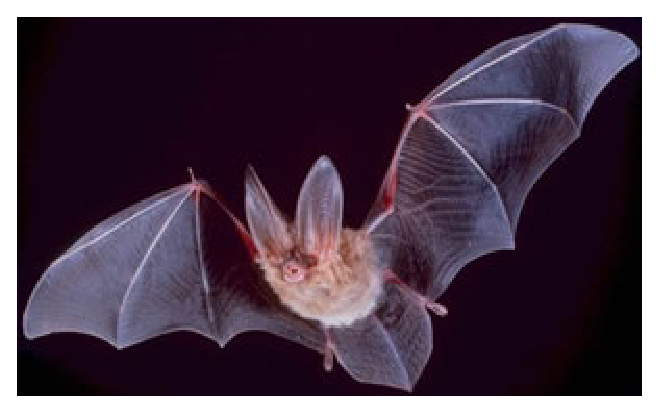
\includegraphics[width=.45\linewidth]{figs/bat_b.eps}\hspace*{0.04in}
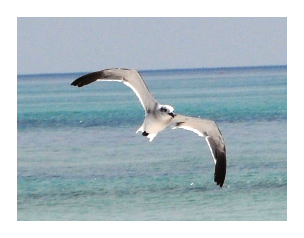
\includegraphics[width=.36\linewidth]{figs/gull2_b.eps}\\
\end{center}
\vspace{-.1in}

\caption
{
Note how a picture that was created or imported differently has a different
space between caption and image than the line drawing in Figure
\protect\ref{pg1}. (Left) Bat flight is being studied as part of an
Air Force Office of Scientific Research Multidisciplinary
University Research Initiative project.
Image credit: mime.oregonstate.edu/news/story/2103, (Right)
Morphing gull wings.
{\em Note how the URL spills too far to the right in the
list of figures. This type of margin infraction must be
corrected manually.}}
\label{batgull2}
\end{figure}



Note that imported pictures that have white space on their margins
will look
as if they are placed incorrectly. For such pictures,
make a note on the printout that goes to format checking.



\section{Tables}

Tables pretty much act like figures. Table~\ref{tablelabel}
is an example of a small table.


\begin{table}[h]
\cprotect\caption{A sample table. If there are no tables,
comment out the \verb+% this contains:
% list of tables
%DO NOT CHANGE IT.





\newpage

% lists of figures and tables
\addcontentsline{toc}{chapter}{LIST OF TABLES}
\begin{singlespace}

%%%\singlespacing
% This configures the space before the title
\renewcommand{\cftbeforelottitleskip}{.6in}%{\SpaceBeforeChapter}
% this configures the space after the title
\renewcommand{\cftafterlottitleskip}{1em}
% This makes the title LIST OF TABLES, centered in bfseries
\renewcommand{\listtablename}{LIST OF TABLES}
\renewcommand{\cftlottitlefont}{\hfill\large\bfseries}
\renewcommand{\cftafterlottitle}{\hfill}

\setlength{\cftparskip}{1.0\baselineskip}%{1.6667\baselineskip}
\renewcommand{\cfttabpresnum}{Table~}
% This will correct the indent so the above added text doesn't distort it

\newlength{\mylenTable}
\settowidth{\mylenTable}{\cfttabpresnum\cfttabaftersnum}
%\addtolength{\cftfignumwidth}{\mylenFigure}
\hyphenpenalty=100000

%% This makes it double space between entries, but single space is turned on already, so it will single space wrapped entries
%\setlength{\cftparskip}{1.0\baselineskip}%{1.6667\baselineskip}
\listoftables
\end{singlespace}



+ command in
\verb+thesis.tex+.
{\em Note how the "include" spills too far to the right in the
list of figures. This type of margin infraction must be
corrected manually.}
}
\vspace{12pt}
\label{tablelabel}
\centerline{
\begin{tabular}{|l|l|r|}
\hline
$p$ & $q$ & $p\Rightarrow q$ \\
\hline
F   & F   & T \\
\hline
F   & T  & T \\
\hline
T  & F   & F  \\
\hline
T  & T  & T  \\
\hline
\end{tabular}
}
\end{table}


For tables, the title is to be placed above the table,
which is done by putting the \verb+\caption+ command
above the table.
To get enough space between the caption and the table,
use \verb+\vspace{12pt}+ to add space.
For professional-looking tables, you'll want to minimize
the number of lines used as done in Table~\ref{tablelabel2}.

\begin{table}[h]
\caption{Another sample table and another fun rule:
Entries in the list of tables/figures
should have at least 3 dots in the dotted
line between entry and page number. Unless there is
an unfortunate spill, which would need to be fixed anyway,
\LaTeX \ should do this automatically.
}
\label{tablelabel2}
\vspace{12pt}
\centering
\begin{tabular}{l l  r}
\toprule
$p$ & $q$ & $p\Rightarrow q$ \\
\midrule
F   & F   & T \\
F   & T  & T \\
T  & F   & F  \\
T  & T  & T  \\
\bottomrule
\end{tabular}
\end{table}


\addtocontents{lot}{So the entries above would need to be fixed by
rewording to eliminate the spills.
(And entries like this one are not permissible.)
\\
~\\
}

\addtocontents{lot}{Also note that to
shrink the gap between the dotted line and the
end of the entry, you should put the closing parenthesis
$\} $ of the caption command right after the last work of the
caption, not on the next line. Compare the entries for
Table \protect\ref{tablelabel} (bad)
and for Figure \protect\ref{batgull2} on the next page.
}


\section{Note on Sections}

If a chapter has only one section, omit the sectioning command.
So for this chapter, I had the choice to omit the section heading
``table" or to explain the reasoning in this short ``section."


\addtocontents{toc}{\protect\renewcommand{\protect\cftchappresnum}{APPENDIX } }

\chapter{CONCLUSIONS}\label{chap6:conclusions}

Put your conclusions here. 


The quick brown fox jumped over the lazy dog.
(I'm so tired of animal acts.)
The quick brown fox jumped over the lazy dog.
(I'm so tired of animal acts.)
The quick brown fox jumped over the lazy dog.
(I'm so tired of animal acts.)
The quick brown fox jumped over the lazy dog.
(I'm so tired of animal acts.)
The quick brown fox jumped over the lazy dog.
(I'm so tired of animal acts.)
The quick brown fox jumped over the lazy dog.
(I'm so tired of animal acts.)
The quick brown fox jumped over the lazy dog.
(I'm so tired of animal acts.)
The quick brown fox jumped over the lazy dog.
(I'm so tired of animal acts.)
The quick brown fox jumped over the lazy dog.
(I'm so tired of animal acts.)
The quick brown fox jumped over the lazy dog.
(I'm so tired of animal acts.)



The quick brown fox jumped over the lazy dog.
(I'm so tired of animal acts.)
The quick brown fox jumped over the lazy dog.
(I'm so tired of animal acts.)
The quick brown fox jumped over the lazy dog.
(I'm so tired of animal acts.)
The quick brown fox jumped over the lazy dog.
(I'm so tired of animal acts.)
The quick brown fox jumped over the lazy dog.
(I'm so tired of animal acts.)
The quick brown fox jumped over the lazy dog.
(I'm so tired of animal acts.)
The quick brown fox jumped over the lazy dog.
(I'm so tired of animal acts.)
The quick brown fox jumped over the lazy dog.
(I'm so tired of animal acts.)
The quick brown fox jumped over the lazy dog.
(I'm so tired of animal acts.)
The quick brown fox jumped over the lazy dog.
(I'm so tired of animal acts.)



The quick brown fox jumped over the lazy dog.
(I'm so tired of animal acts.)
The quick brown fox jumped over the lazy dog.
(I'm so tired of animal acts.)
The quick brown fox jumped over the lazy dog.
(I'm so tired of animal acts.)
The quick brown fox jumped over the lazy dog.
(I'm so tired of animal acts.)
The quick brown fox jumped over the lazy dog.
(I'm so tired of animal acts.)
The quick brown fox jumped over the lazy dog.
(I'm so tired of animal acts.)
The quick brown fox jumped over the lazy dog.
(I'm so tired of animal acts.)
The quick brown fox jumped over the lazy dog.
(I'm so tired of animal acts.)
The quick brown fox jumped over the lazy dog.
(I'm so tired of animal acts.)
The quick brown fox jumped over the lazy dog.
(I'm so tired of animal acts.)


 % Conclusions
%MUST PUT LAST CHAPTER IN THIS FILE TO HAVE FIRST APPENDIX CALLED
%APPENDIX, NOT CHAPTER IN TABLE OF CONTENTS



\appendix


\renewcommand{\thefigure}{\Alph{chapter}.\arabic{figure}}
\renewcommand{\thetable}{\Alph{chapter}.\arabic{table}}




\chapter{APPENDICES (IF DESIRED)}\label{append1}

\clearpage


{\bf Put your appendices here. All codes stay the same, except that 
the first page of an appendix should only have the 
headings, so follow $\setminus $chapter with a 
$\setminus $clearpage. Codes in phd\underline{~}thesis.tex
take care of naming a $\setminus $chapter an ``APPENDIX."}

From Louisiana Tech's
``GUIDELINES FOR THE
PREPARATION AND SUBMISSION
OF YOUR THESIS OR DISSERTATION"
(see \cite{guide})



\begin{itemize}
\item
Appendices are optional. They must contain extra, relevant material such as
questionnaires, surveys, tables, figures, computer data, and letters of permission
to reprint copyrighted material. These optional appendices must be listed in the
Table of Contents, conforming to the format used there. They must also be
formatted in the document in such a way that they are consistent with the other
main divisions.
\item
Appendices must be cited in the Body of the document.
\item
All material in appendixes must be numbered consecutively, within the required
margins, and on the same paper used throughout the document.
\item
All appendices must have a title page. The title page of each Appendix must have
the Arabic page number centered between the left and right margins between $1/2$
inch and 1 inch from the bottom edge of the page. Place the Arabic page number
at the top right of subsequent pages of each Appendix.
\item
The Title page must have the word APPENDIX typed in all capital letters 2
inches from the top of the page followed by an informative title in all capital
letters. If there is more than one appendix, then label the first title page as
APPENDIX A, the second APPENDIX B, and so on, providing an
informative title for each appendix.
\end{itemize} %Comment out if there are no appendices


% Bibliography
\addcontentsline{toc}{chapter}{BIBLIOGRAPHY}
\renewcommand{\bibname}{\MakeUppercase{Bibliography}}
\begin{singlespace}
%\baselineskip = 24pt



\begin{thebibliography}{99}
\setlength{\itemsep}{0.3in}

\bibitem{bib1}
Author A,
First entry in the bibliography.


For bibliographies single space the entries and put a double space between
entries.

BTW, \LaTeX \ measurements are
as follows. Double space: 24pt = 0.3in in between lines.
Triple space: 36pt = 0.6in between lines


\bibitem{bib2}
Author B,
Second entry in the bibliography.

\bibitem{bib3}
Caution:
Use the formatting style that is common in your discipline.
{\em None of the entries in this file should be considered a sample entry.}




\bibitem{guide}
Louisiana Tech Univervsity,
GUIDELINES FOR THE
PREPARATION AND SUBMISSION
OF YOUR THESIS OR DISSERTATION,
available at
{\tt http://www.latech.edu/graduate\underline{~}school/thesis\underline{~}dissertations/index.shtml}

(margin infraction!)


\bibitem{MiKTeX}
MiKTeX, available at
{\tt http://miktex.org/}


\bibitem{warning}
Do {\bf not} split bibliography entries between two pages.
Use $\setminus $clearpage commands to introduce hard page breaks
as necessary.
I tried to put in a split entry, but it may well be that
\LaTeX \ avoids bad splits automatically.


\bibitem{texcad}
\TeX CAD, available at {\tt http://texcad.sourceforge.net/}



\bibitem{TeXnicCenter}
TeXnicCenter, available at
{\tt http://www.texniccenter.org/}

\bibitem{WinEdt}
WinEdt, available at
{\tt http://winedt.com/}




\end{thebibliography}

%Note: There also was a change in the code for the bibliography so that 
%entries are single spaced with a double space between entries.

%\baselineskip = 24pt
\end{singlespace}

% thesis_vita.tex
% this some biographical information to go into the vita portion
% of my dissertation.
\chapter*{VITA (IF REQUIRED)}
\addcontentsline{toc}{chapter}{VITA}

\begin{itemize}
\item
The Vita is a one-page biographical sketch of the author written in paragraph
form and in 3rd person. It is the last item of the document and must appear in the
Table of Contents.
\item
The heading must have identical font, value, size, and position/location in the
page as other major headings.
\end{itemize}

\end{document}
